This chapter contains theoretical information about the paper's domain, deep learning,
and the principal model used, autoencoders.
Of course, before starting looking in its domain,
we should start with the basics, namely, machine learning.
\section{What is Machine Learning?}

Machine learning is one of many subfields of artificial intelligence,
the science of getting the computer to learn from experience
without being explicitly programmed to do so,
improving their ability to think, plan, decide, etc. \cite{whatIsML}.\par
Algorithms in this area are different in their approach, the type of data they input and output,
and the type of problem they are learning to
solve, but, despite all differences, they are based on the same idea that there are some
generic algorithms that can discover patterns,
without having to write code; instead, they build their own logic on the data fed to them.
% \vspace{0.5cm}

% @HERE
\section{Machine Learning Styles}
When studying machine learning, one can identify a plethora of algorithms,
each unique in its approach and purpose, but all of them can be classified
based on the learning style. Therefore, there can be grouped into four main categories:
\begin{itemize}
    \item \textbf{Supervised Learning}
    \item \textbf{Unsupervised Learning}
    \item \textbf{Semi-supervised Learning}
    \item \textbf{Reinforcement Learning}
\end{itemize}
\vspace{0.5cm}

% @HERE
\subsection{Supervised Learning}
In supervised learning, given a set of example input-output pairs,
the job of the algorithms is to approximate a function that maps from input to output \cite{amai}.
It is called supervised learning because human experts act as the teacher,
where they serve the computer with training data containing the input and
also provide the correct output, from which the computer should be able to observe patterns.
As seen depicted in Figure\emph{~\ref{fig:supervised}},
the algorithm should be able to predict the output when given new inputs,
based on the function that it approximates \cite{typesMLMedium}.

\begin{figure}[h]
    \centering
    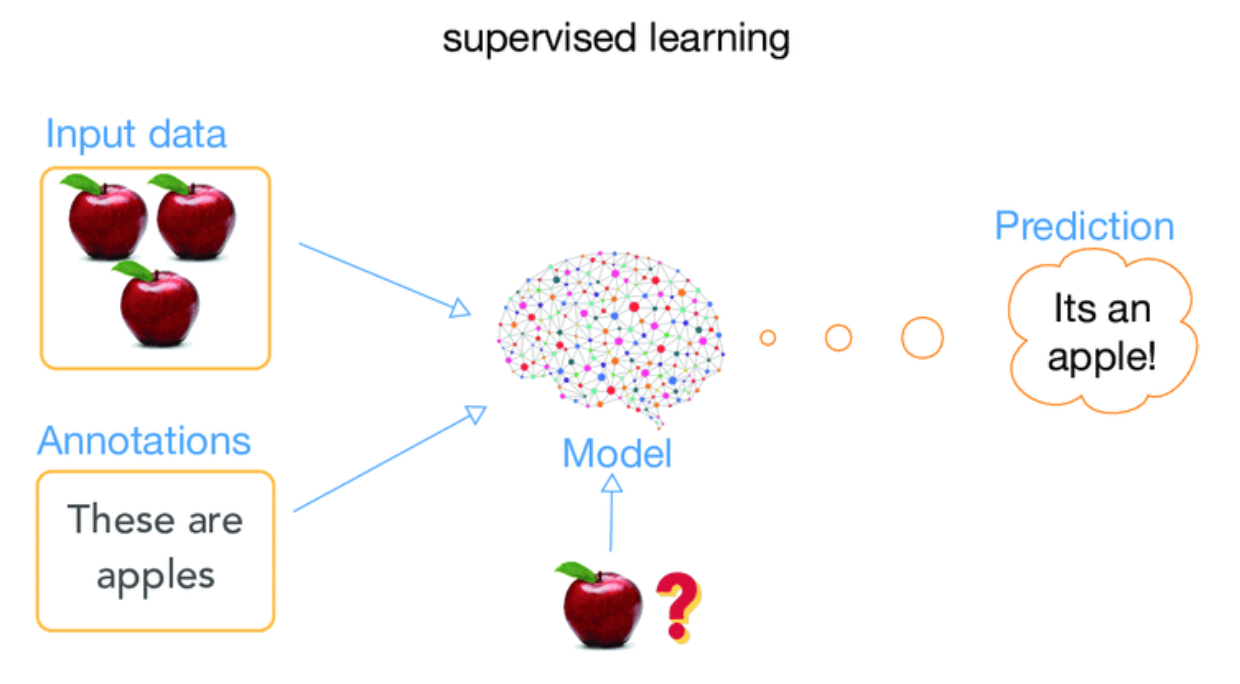
\includegraphics[width=1\textwidth]{supervised_learning}
    \caption{\emph{Supervised algorithm predicting new output data given new input  \cite{typesML}}}
    \label{fig:supervised}
\end{figure}

Furthermore, supervised machine learning algorithms can also
be grouped based on the type of problem they intend to solve.
Having said that, there are classification and regression algorithms.

% @HERE Classification
Classification algorithms solve problems in which the input data has
been labelled in different classes or categories,
meaning that the goal is to predict discrete values
such as $\{0, 1\}$, $\{2, 4, 6, 8\dots\}$, $\{cat, dog\}$, $\{spam, normal\}$, etc \cite{typesMLMedium}.

% @HERE Regression
Regression algorithms, on the other hand, solve problems in which the output variable
is a real value, meaning that the goal is to predict continuous values based on the
input data, such as predicting house prices based on their size and location \cite{typesMLMedium}.

\begin{figure}[h]
    \centering
    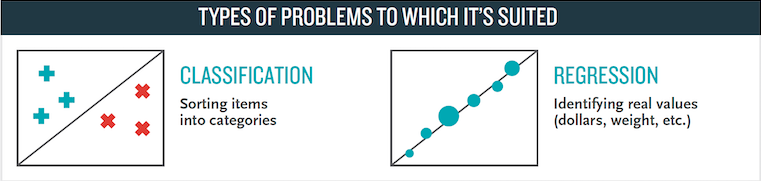
\includegraphics[width=0.8\textwidth]{regression_classification}
    \caption{\emph{Classification(left) and Regression(right) visualization  \cite{bigDataR}}}
    \label{fig:regression_classification}
\end{figure}


\subsection{Unsupervised Learning}
In unsupervised learning, the job of the algorithms is to observe patterns in
the structure of the given data even though no explicit feedback is supplied \cite{amai}.
There is no human factor implied in the learning process,
hence the name of unsupervised learning.
As shown in Figure\emph{~\ref{fig:unsupervised}}, they should be able to identify the underlying
structure in the given data, to better understand it \cite{bigDataR}.

\begin{figure}[h]
    \centering
    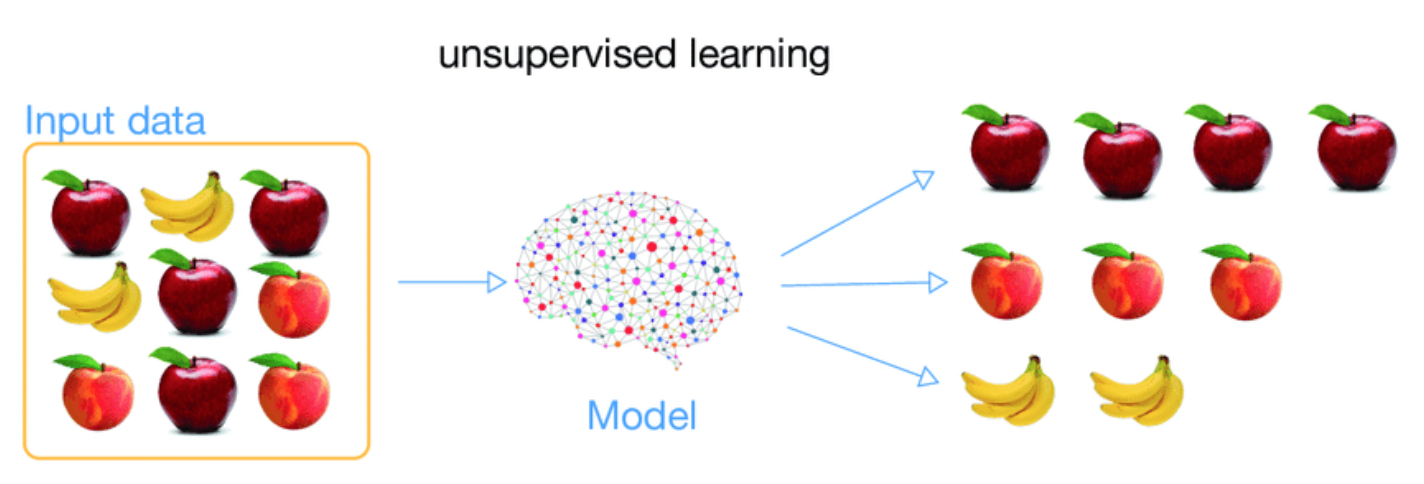
\includegraphics[width=1\textwidth]{unsupervised_learning}
    \caption{\emph{Unsupervised algorithm grouping data by their observed features \cite{typesML}}}
    \label{fig:unsupervised}
\end{figure}

The same as supervised learning, unsupervised algorithms can also be grouped
based on the type of problem they intend to solve. Provided that,
there are clustering and low-dimensional embedding algorithms \cite{amai}.

%  @HERE clustering
Clustering algorithms try to solve problems by grouping the input data
into different segments based on similarities learned,
such as grouping customers by purchasing behaviour \cite{brownlee2016master}.


% @HERE dimensionality reduction
Low-dimensional embedding, also called dimensionality reduction,
is a technique in which complex data, that is difficult to describe
(data that needs more than two or three dimensions to represent)
is reduced to a lower number of dimensions,
wherein the machine learning algorithms can help
since they can learn the internal structure inside our data, furthermore,
transcribing it to an easier way of interpreting it \cite{amai}.


\subsection{Semi-supervised Learning}
Semi-supervised learning algorithms lie between the aforementioned categories.
They intend to solve problems where you have a large amount of data but only some labelled.
A lot of machine learning problems are using this technique for the reason that
labelled data can be expensive or time-consuming to obtain,
in contrast to unlabelled data that is much easier to acquire \cite{brownlee2016master}.

As shown in Figure Figure\emph{~\ref{fig:semi_supervised_learning}}, one can use an initial classifier on the labelled data,
classify based on the features learned previously, the unlabelled data,
retrain the classifier with the whole dataset,
then use it to predict new outputs given new input data, ideally obtaining a better model \cite{lotte2015}

\begin{figure}[h]
    \centering
    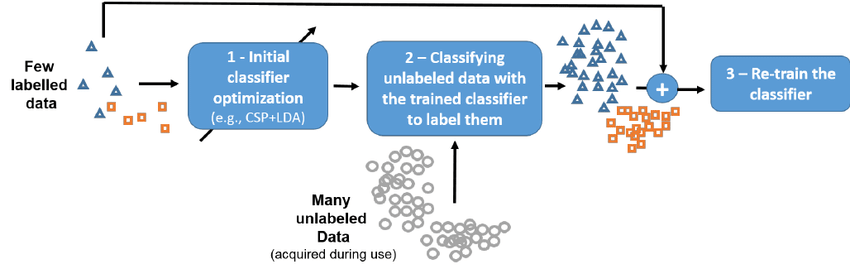
\includegraphics[width=1\textwidth]{semi_supervised_learning}
    \caption{\emph{Semi-supervised approach on data classification \cite{lotte2015}}}
    \label{fig:semi_supervised_learning}
\end{figure}

\subsection{Reinforcement Learning}
Reinforcement learning algorithms are based on a system of type reward-punishment,
where the job of the algorithm is to iteratively interact with its environment,
making actions in such a manner that will maximize the rewards or minimize the punishments.
To put it another way, in reinforcement learning,
the software learns from its past experiences allowing it to develop an optimal
behaviour within a specific setting, where it aims to increase its performance \cite{typesMLMedium}.

\begin{figure}[h]
    \centering
    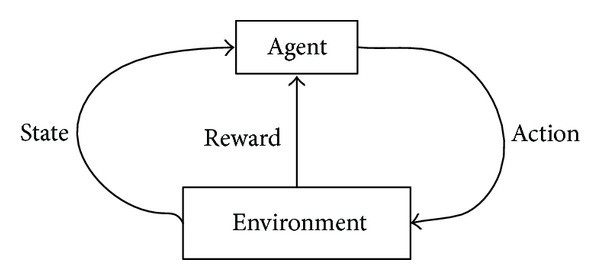
\includegraphics[width=1\textwidth]{reinforcement_learning}
    \caption{\emph{Scheme of how reinforcement algorithms work \cite{typesMLMedium}}}
    \label{fig:reinforcement_learning}
\end{figure}

Figure\emph{~\ref{fig:reinforcement_learning}} is a visual representation of how reinforcement learning works. The algorithm
(called the "agent" in the picture), takes action in the environment,
which will possibly trigger a reward. After that, the state is updated,
and when deciding its next action, it will take into account its last state and the
result of the previous action.

\section{ANNs and how they work}
One of the main types of machine learning algorithms that are vastly used is
artificial neural networks or ANNs.
They are structured as weighted graphs, modelled after the
human brain where each node represents a neuron and each
edge represents the synapses of the neural network.
The weight of each edge determines how powerful the synapse is.
The neurons are distributed in groups named layers.
Neurons can form synapses only with neurons from other layers \cite{understandingANN}.

\subsection{Artificial neurons and activation function}

The smallest unit of an artificial neural network is the \textbf{artificial neuron},
namely the nodes of the graph. It is the place where the computation happens:
a node merges the input data by doing their weighted sum, to dampen or amplify the input.
Further, the result will be given to a so-called \textbf{activation function} whose purpose is to
determine whether or not the neural signal will be passed on to the next neurons or not \cite{pathMind}.
A more detailed explanation of the subject can be seen in Figure\emph{~\ref{fig:artificial_neuron}}.

\begin{figure}[h]
    \centering
    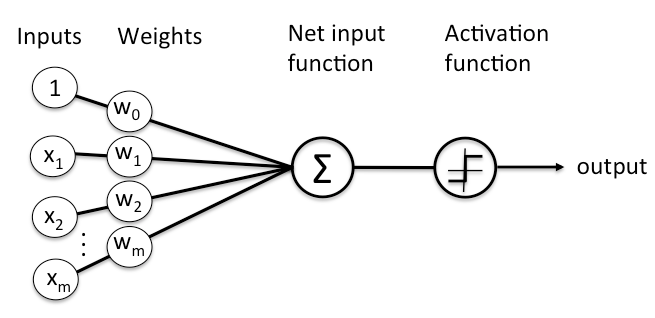
\includegraphics[width=1\textwidth]{artificial_neuron}
    \caption{\emph{Anatomy of an artificial neural network \cite{pathMind}}}
    \label{fig:artificial_neuron}
\end{figure}

The aforesaid \textbf{activation function} is a mathematical expression that helps
the ANN to add non-linearity to itself. With more and bigger datasets,
the patterns that need to be identified become more complex.
With the help of these types of function, the input is much easier to analyze and interpret.

\begin{itemize}
    \item{
          \textbf{zero-centered}: output should be symmetrical
          at zero so that it does not move to a particular direction;
          }
    \item{
          \textbf{computationally inexpensive}: the function is called for every layer
          for each input data, meaning that it could be invoked thousands of times.
          Therefore, they should not be computationally expensive;
          }
    \item{
          \textbf{differentiable}: at the core of almost every machine algorithm lies
          an optimization algorithm. One of the most popular
          approaches is the gradient descent algorithm in which one of the most essential
          features is that the function used needs to be differentiable;
          this idea will be discussed in detail in a subsequent paragraph;
          }
\end{itemize}



\subsection{Backpropagation and gradient descent}

\textbf{Backpropagation} describes how machine algorithms learn.
As show in Figure\emph{\ref{fig:backpropagation}},
after the data traverses the neural network in a forward manner,
propagating the signals through the neurons,
the algorithm will go in reverse adjusting each weight for each node and its links \cite{Goodfellow-et-al-2016}.
This technique is called backpropagation of errors, or simply,
backpropagation and is the learning engine of the most ANN's.

\begin{figure}[h]
    \centering
    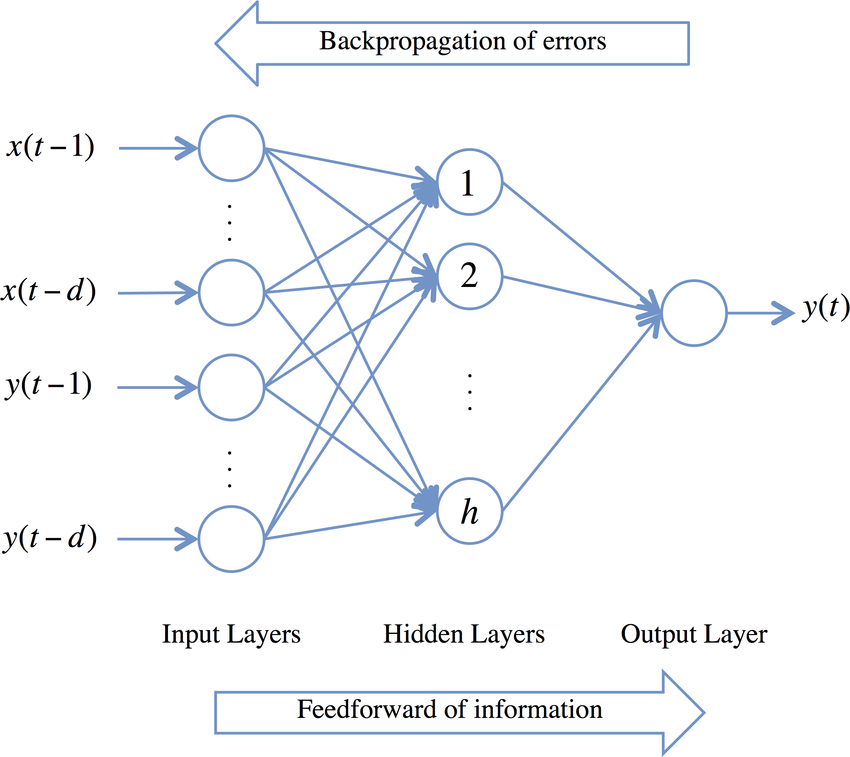
\includegraphics[width=1\textwidth]{backpropagation}
    \caption{\emph{Feedforward Backpropagation Neural Network architecture. \cite{backpropagation}}}
    \label{fig:backpropagation}
\end{figure}

The \textbf{gradient descent}, as mentioned before,
is an optimization algorithm best-used to find the (local) minimum value for a function \cite{brownlee2016master}.
Hence, it can be used to reduce the errors in our algorithm,
since the training of a neural network is just the process of finding the set of weights and other
parameters in such a fashion that the errors(differences) between our expected and actual results are minimum.
Hence, the gradient descent is used to compute the errors of our algorithm, that will be later backpropagated
through the ANN.


\subsection{Layers of ANNs}
Multiple artificial neurons are grouped in \textbf{layers};
the purpose of each one is to apply a non-linear
transformation of the input from one vector space to another \cite{appliedDeepLearning}.
As you can see in \emph{\ref{fig:ann_structure}} there are three types of layers in an artificial neural network:
\begin{itemize}[]
    \item{ Input layer
          \begin{adjustwidth}{1cm}{}
              This layer of a neural network is the very beginning of the ANN’s workflow, bringing the initial data into the system for
              further processing by subsequent layers of artificial neurons \cite{inputLayer}.
          \end{adjustwidth}
          }
    \item{ Hidden layer
          \begin{adjustwidth}{1cm}{}
              Any layer between the output and the input layer is considered to be a hidden layer.
              The number of neurons they contain and also their number can vary.
              Their role is to take in a set of weighted inputs and produce an output through an activation function \cite{hiddenlayer}.
          \end{adjustwidth}
          }
    \item{ Output layer
          \begin{adjustwidth}{1cm}{}
              This layer of a neural network is the last layer of neurons that produces given outputs for the program.
              They usually are made much like any other artificial neuron, but they may be observed in a different way,
              the output layer coalesces and concretely produces the end result \cite{outputLayer}.
          \end{adjustwidth}
          }
\end{itemize}
\begin{figure}[h]
    \centering
    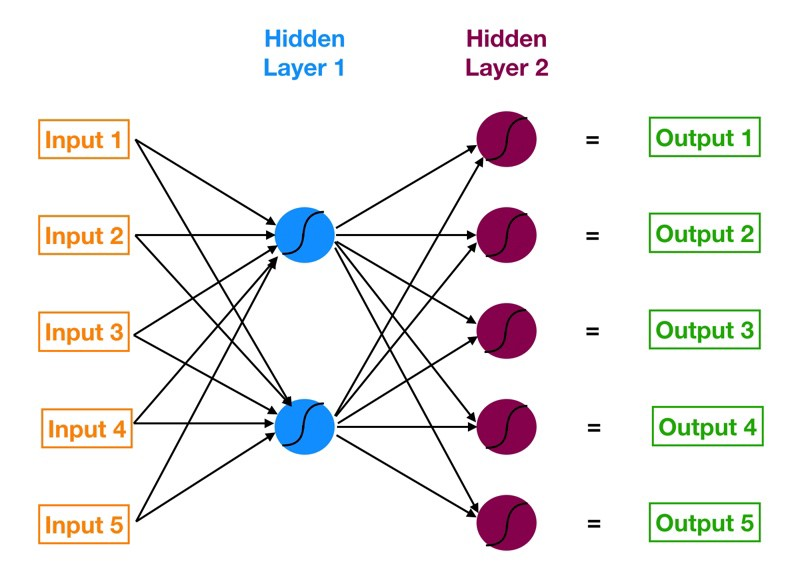
\includegraphics[width=1\textwidth]{ann_structure}
    \caption{\emph{Neural network with one hidden layer \cite{understandingANN}}}
    \label{fig:ann_structure}
\end{figure}


\section{What is Deep Learning?}

Deep learning is a subfield of machine learning that contains a collection of ANNs that are known for
their capability on learning unsupervised from data that is unstructured or unlabeled,
also known as deep neural learning or deep neural network.

A second classification we can make on ANNs is based on the relationships between their nodes.
Then, neural networks can be recurrent or feedforward;
the first one does not have any loops in its graph and can be organized in layers.
A deep neural network is a feedforward ANN with many hidden layers.

A visual representation of the aforementioned is the Figure\emph{~\ref{fig:deep_vs_normal}}
wherein we could see the differences between a simple feedforward ANN with one
hidden layer(left) and a deep neural network with three hidden layers
\begin{figure}[h]
    \centering
    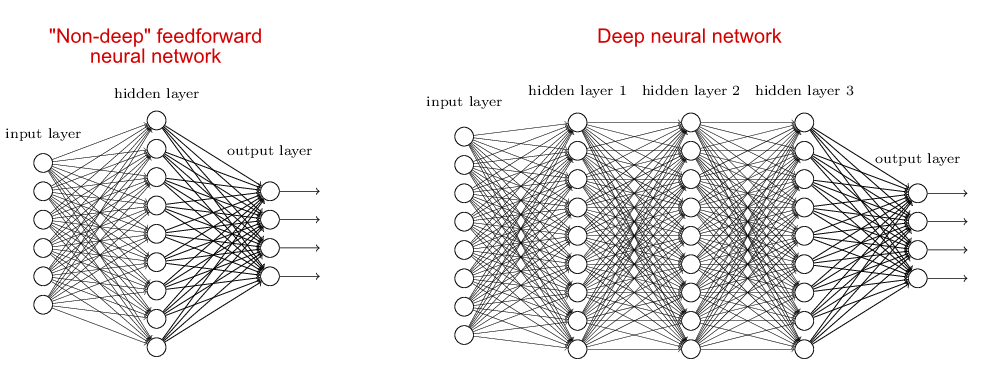
\includegraphics[width=1\textwidth]{deep_vs_normal_ann}
    \caption{\emph{Difference between a Non-deep ANN(left) and a deep ANN(right) \cite{deepLearningBook}}}
    \label{fig:deep_vs_normal}
\end{figure}

Deep learning is an area in machine learning that achieves state-of-the-art
results by learning to represent the world "as a nested hierarchy of concepts,
with each concept defined in relation to simpler concepts,
and more abstract representations computed in terms of less abstract ones" \cite{Goodfellow-et-al-2016}


\section{Autoencoders and how they learn}
WIP
